% !TEX root = ../report.tex

\section{Logical View}
\label{sec:viewlogical}

% Logical view : The logical view is concerned with the functionality that the system provides to end-users. UML Diagrams used to represent the logical view include Class diagram, Communication diagram, Sequence diagram.

\begin{figure}[H]
\caption{An high-level overview of the Docker architecture. Source: \cite{dockerarchi}.}
\centering
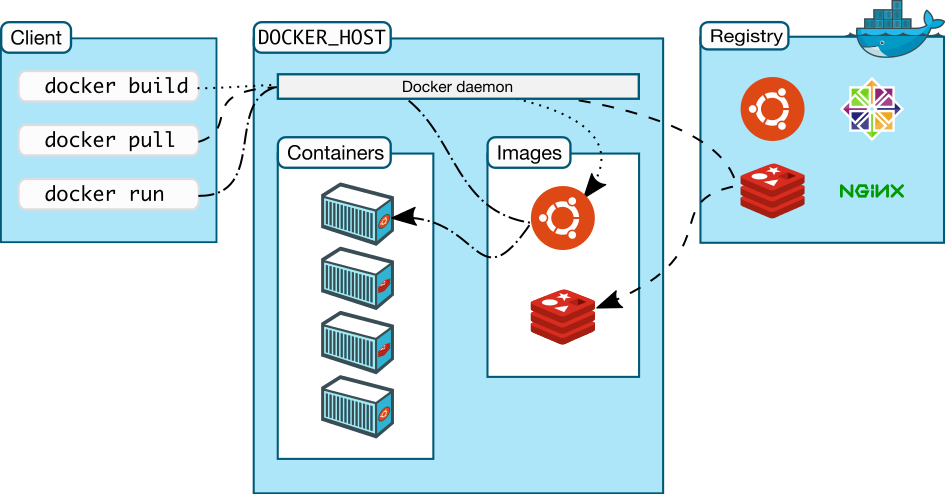
\includegraphics[scale=0.4]{4-softwarearch/images/architecture.png}
\end{figure}
Docker uses a client-server architecture. The client (a command-line tool) acts as the primary user interface and talks to the Docker daemon. The daemon is a background process which does all the heavy lifting, e.g. the building and running of the containers.

%Docker uses a client-server architecture. The Docker client talks to the Docker daemon, which does the heavy lifting of building, running, and distributing your Docker containers. Both the Docker client and the daemon can run on the same system, or you can connect a Docker client to a remote Docker daemon. The Docker client and daemon communicate via sockets or through a RESTful API.

\subsection{Client}

\subsection{Server / Daemon}

\subsubsection{Containers}
\subsubsection{Images}


\subsection{Registry}